\documentclass[letterpaper,12pt]{article}
\usepackage[dvips]{epsfig,geometry}
%\usepackage{multicol}
%\usepackage{fancyhdr}
%\pagestyle{fancy}
\usepackage{nicefrac}
\usepackage{indentfirst}
\usepackage{amssymb}
\usepackage{color}
\usepackage{enumerate}
\usepackage{comment}
\usepackage{overcite}
\usepackage{citesort}
\usepackage{geometry}
\usepackage{amsmath}
\usepackage[]{caption}
%\usepackage{aip}
\usepackage{bm}
\usepackage{wrapfig}
\usepackage{subfigure}
\geometry{letterpaper,textwidth=6.5in,textheight=9.0in,left=1.in,right=1in,top=1in}
\setlength{\parindent}{0.25in}
\renewcommand{\baselinestretch}{1.25}
\baselineskip = 13pt

%-------------------------------------------------------------------------------------------------------------------
%COMMANDS
%-------------------------------------------------------------------------------------------------------------------
\newcommand{\two}{\mspace{-2.0mu}}
\newcommand{\four}{\mspace{-4.0mu}}
\newcommand{\plus}{\mspace{-4.5mu}+\mspace{-3.5mu}}
\newcommand{\minus}{\mspace{-4.5mu}-\mspace{-3.5mu}}
\newcommand{\pp}{'\mspace{-2.0mu}'}

\newcommand{\xlb}[4]{#1\ifthenelse{\equal{#2}{0}}{}{_{\alpha #2}}
\mspace{-2.0mu}\genfrac{(}{)}{0pt}{1}{\ifthenelse{\equal{#3}{0}}{0}{l #3}} {\ifthenelse{\equal{#4}{0}}{0}{b #4}}}

\newcommand{\xkv}[4]{#1\mspace{-5.0mu}\left(\mspace{-8.0mu}\begin{smallmatrix}#2\four{}\four{}\mspace{-8.0mu}&\pmb{\kappa}#3\\&\nu #4\end{smallmatrix}\mspace{-5.0mu}\right)}

\newcommand{\evect}[6]{#1\mspace{-4.0mu}\left(\mspace{-8.0mu}\begin{smallmatrix}#2\mspace{-8.0mu}&\pmb{\kappa} #3 &b #5\\&\nu #4 &\alpha #6\end{smallmatrix}\mspace{-5.0mu}\right)}

\newcommand{\varmat}[8]{\mspace{-5.0mu}\left(\mspace{-8.0mu}\begin{smallmatrix}\ifthenelse{\equal{#3}{0}}{\mspace{-8.0mu}&b_{#1}&b_{#2}\\&\alpha_{#1}&\alpha_{#2}} {\ifthenelse{\equal{#7}{0}}{#1\mspace{-8.0mu}&\pmb{\kappa}#2#3\mspace{-8.0mu}&\pmb{\kappa}#4#5\mspace{-8.0mu}&\pmb{\kappa}#6\\&\nu#2&\nu#4&\nu#6} {#1\mspace{-8.0mu}&\pmb{\kappa}#2#3\mspace{-8.0mu}&\pmb{\kappa}#4#5\mspace{-8.0mu}&\pmb{\kappa}#6#7\mspace{-8.0mu}&\pmb{\kappa}#8\\&\nu#2&\nu#4&\nu#6&\nu#8}}\end{smallmatrix}\mspace{-5.0mu}\right)}

\newcommand{\EXP}[1]{\exp\mspace{-5.0mu}\left[#1\right]\mspace{-3.0mu}}

\newcommand{\tpp}[2]{\left(\mspace{-2.0mu}\xkv{\omega}{}{}{}#1\xkv{\omega}{}{'}{'}#2\xkv{\omega}{}{\pp}{\pp}\mspace{-2.0mu}\right)}

\newcommand{\be} {\begin{eqnarray}}
\newcommand{\ee} {\end{eqnarray}}
\newcommand{\f}[2]{\ensuremath{\frac{\displaystyle{#1}}{\displaystyle{#2}}}}
\newcommand{\lr}[1]{\langle{#1}\rangle}

\newcommand{\SUM}[2]{\ifthenelse{\equal{#1}{0}}{\sum_{\alpha_{#2},b_{#2},l_{#2}}^{3,n,N}} {\ifthenelse{\equal{#1}{1}}{\sum_{\alpha_{#2},b_{#2}}^{3,n}}{\sum_{\pmb{\kappa}#2,\nu#2}^{N,3n}}}}

\newcommand{\SUMprime}[2]{\ifthenelse{\equal{#1}{0}}{\sum_{\alpha_{#2},b_{#2},l_{#2}}^{3,n,N}} {\ifthenelse{\equal{#1}{1}}{\sum_{\alpha_{#2},b_{#2}}^{3,n}}{\sum_{\pmb{\kappa}^{'}#2,\nu#2}^{N,3n}}}}

\newcommand{\SUMalpha}[2]{\ifthenelse{\equal{#1}{0}}{\sum_{\alpha_{#2}}^{3}} {\ifthenelse{\equal{#1}{1}}{\sum_{\alpha_{#2},b_{#2}}^{3,n}}{\sum_{\pmb{\kappa}#2,\nu#2}^{N,3n}}}}

\newcommand{\SUMalphap}[2]{\ifthenelse{\equal{#1}{0}}{\sum_{\alpha'_{#2}}^{3}} {\ifthenelse{\equal{#1}{1}}{\sum_{\alpha'_{#2},b'_{#2}}^{3,n}}{\sum_{\pmb{\kappa}#2,\nu#2}^{N,3n}}}}

\newcommand{\SUMb}[2]{\ifthenelse{\equal{#1}{0}}{\sum_{b_{#2}}^{n}} {\ifthenelse{\equal{#1}{1}}{\sum_{\alpha_{#2},b_{#2}}^{3,n}}{\sum_{\pmb{\kappa}#2,\nu#2}^{N,3n}}}}

\newcommand{\SUMbp}[2]{\ifthenelse{\equal{#1}{0}}{\sum_{b'_{#2}}^{n}} {\ifthenelse{\equal{#1}{1}}{\sum_{\alpha'_{#2},b'_{#2}}^{3,n}}{\sum_{\pmb{\kappa}#2,\nu#2}^{N,3n}}}}

\newcommand{\SUMl}[2]{\ifthenelse{\equal{#1}{0}}{\sum_{l_{#2}}^{N}} {\ifthenelse{\equal{#1}{1}}{\sum_{\alpha_{#2},b_{#2}}^{3,n}}{\sum_{\pmb{\kappa}#2,\nu#2}^{N,3n}}}}

\newcommand{\SUMlp}[2]{\ifthenelse{\equal{#1}{0}}{\sum_{l'_{#2}}^{N}} {\ifthenelse{\equal{#1}{1}}{\sum_{\alpha'_{#2},b'_{#2}}^{3,n}}{\sum_{\pmb{\kappa}#2,\nu#2}^{N,3n}}}}

\newcommand{\abcdt}[5]{\mspace{-4.0mu}\left(\mspace{-8.0mu}\begin{smallmatrix}&\ifthenelse{\equal{#1}{}}{a}{#1}&\ifthenelse{\equal{#3}{}}{c}{#3}\\&\ifthenelse{\equal{#2}{}}{b}{#2}&\ifthenelse{\equal{#4}{}}{d}{#4}\end{smallmatrix}\mspace{-2.0mu};\ifthenelse{\equal{#5}{}}{t}{#5}\right)}

\newcommand{\abcd}[4]{\mspace{-4.0mu}\left(\mspace{-8.0mu}\begin{smallmatrix}&\ifthenelse{\equal{#1}{}}{a}{#1}&\ifthenelse{\equal{#3}{}}{c}{#3}\\&\ifthenelse{\equal{#2}{}}{b}{#2}&\ifthenelse{\equal{#4}{}}{d}{#4}\end{smallmatrix}\mspace{-3.0mu}\right)}

\newcommand{\abt}[3]{\mspace{-4.0mu}\left(\mspace{-8.0mu}\begin{smallmatrix}&\ifthenelse{\equal{#1}{}}{a}{#1} \\&\ifthenelse{\equal{#2}{}}{b}{#2}\end{smallmatrix}\mspace{-2.0mu};\ifthenelse{\equal{#3}{}}{t}{#3}\right)}

\newcommand{\ab}[2]{\mspace{-4.0mu}\left(\mspace{-8.0mu}\begin{smallmatrix}&\ifthenelse{\equal{#1}{}}{a}{#1} \\&\ifthenelse{\equal{#2}{}}{b}{#2}\end{smallmatrix}\mspace{-3.0mu}\right)}

\newcommand{\kvbat}{\mspace{-4.0mu}\left(\mspace{-8.0mu}\begin{smallmatrix} &\pmb{\kappa} &b \\ &\nu &\alpha\end{smallmatrix}\mspace{-2.0mu};t\right)}

\newcommand{\kvbatp}{\mspace{-4.0mu}\left(\mspace{-8.0mu}\begin{smallmatrix} &\pmb{\kappa} &b' \\ &\nu &\alpha'\end{smallmatrix}\mspace{-2.0mu};t\right)}

\newcommand{\kvbaw}{\mspace{-4.0mu}\left(\mspace{-8.0mu}\begin{smallmatrix} &\pmb{\kappa} &b \\ &\nu &\alpha\end{smallmatrix}\mspace{-2.0mu};\omega\right)}

\newcommand{\kvbawp}{\mspace{-4.0mu}\left(\mspace{-8.0mu}\begin{smallmatrix} &\pmb{\kappa} &b' \\ &\nu &\alpha'\end{smallmatrix}\mspace{-2.0mu};\omega\right)}

\newcommand{\kvba}{\mspace{-4.0mu}\left(\mspace{-8.0mu}\begin{smallmatrix} &\pmb{\kappa} &b \\ &\nu &\alpha\end{smallmatrix}\mspace{-3.0mu}\right)}

\newcommand{\kvbap}{\mspace{-4.0mu}\left(\mspace{-8.0mu}\begin{smallmatrix} &\pmb{\kappa} &b' \\ &\nu &\alpha'\end{smallmatrix}\mspace{-3.0mu}\right)}

\newcommand{\kpvba}{\mspace{-4.0mu}\left(\mspace{-8.0mu}\begin{smallmatrix} &\pmb{\kappa}^{'} &b \\ &\nu &\alpha\end{smallmatrix}\mspace{-3.0mu}\right)}

\newcommand{\kva}{\mspace{-4.0mu}\left(\mspace{-8.0mu}\begin{smallmatrix} &\pmb{\kappa} \\ &\nu &\alpha\end{smallmatrix}\mspace{-3.0mu}\right)}

\newcommand{\kvap}{\mspace{-4.0mu}\left(\mspace{-8.0mu}\begin{smallmatrix} &\pmb{\kappa} \\ &\nu &\alpha'\end{smallmatrix}\mspace{-3.0mu}\right)}

\newcommand{\kvb}{\mspace{-4.0mu}\left(\mspace{-8.0mu}\begin{smallmatrix} &\pmb{\kappa} &b \\ &\nu \end{smallmatrix}\mspace{-3.0mu}\right)}

\newcommand{\kvbp}{\mspace{-4.0mu}\left(\mspace{-8.0mu}\begin{smallmatrix} &\pmb{\kappa} &b' \\ &\nu \end{smallmatrix}\mspace{-3.0mu}\right)}

\newcommand{\kvt}{\mspace{-4.0mu}\left(\mspace{-8.0mu}\begin{smallmatrix}&\pmb{\kappa} \\&\nu\end{smallmatrix}\mspace{-2.0mu};t\right)}

\newcommand{\kpvt}{\mspace{-4.0mu}\left(\mspace{-8.0mu}\begin{smallmatrix}&\pmb{\kappa}^{'} \\&\nu\end{smallmatrix}\mspace{-2.0mu};t\right)}

\newcommand{\kvw}{\mspace{-4.0mu}\left(\mspace{-8.0mu}\begin{smallmatrix}&\pmb{\kappa} \\&\nu\end{smallmatrix}\mspace{-2.0mu};\omega\right)}

\newcommand{\kv}{\mspace{-4.0mu}\left(\mspace{-8.0mu}\begin{smallmatrix}&\pmb{\kappa} \\&\nu\end{smallmatrix}\mspace{-3.0mu}\right)}

\newcommand{\lbt}{\mspace{-4.0mu}\left(\mspace{-8.0mu}\begin{smallmatrix}&l \\&b\end{smallmatrix}\mspace{-2.0mu};t\right)}

\newcommand{\lbtp}{\mspace{-4.0mu}\left(\mspace{-8.0mu}\begin{smallmatrix}&l' \\&b'\end{smallmatrix}\mspace{-2.0mu};t\right)}

\newcommand{\lt}{\mspace{-4.0mu}\left(\mspace{-8.0mu}\begin{smallmatrix}&l\end{smallmatrix}\mspace{-2.0mu};t\right)}

\newcommand{\ltp}{\mspace{-4.0mu}\left(\mspace{-8.0mu}\begin{smallmatrix}&l'\end{smallmatrix}\mspace{-2.0mu};t\right)}

\newcommand{\lb}{\mspace{-4.0mu}\left(\mspace{-8.0mu}\begin{smallmatrix}&l \\&b\end{smallmatrix}\mspace{-3.0mu}\right)}

\newcommand{\lbp}{\mspace{-4.0mu}\left(\mspace{-8.0mu}\begin{smallmatrix}&l' \\&b'\end{smallmatrix}\mspace{-3.0mu}\right)}

%-------------------------------------------------------------------------------------------------------------------
%COMMANDS
%-------------------------------------------------------------------------------------------------------------------


%-------------------------------------------------------------------------------------------------------------------
%Begin Doc
%-------------------------------------------------------------------------------------------------------------------

\begin{document}

\title{Thermal Transport in Disordered Materials}

\author{Jason M. Larkin}
\author{Joseph E. Turney}
\author{Alexandre D. Massicotte}
\author{A. J. H. McGaughey}
\affiliation{Department of Mechanical Engineering\\Carnegie Mellon University\\Pittsburgh, PA 15213}

\date{\today}

\begin{abstract}
Thermal transport in disordered materials is not well understood.  For example:


1) Understanding thermal transport in crystalline systems requires detailed knowledge of the phonon properties.

2) Thermal transport in dilute alloys should have significant contribution from phonons.  As the alloy concentration is increased, the vibrational modes should become localized and non-propagating.

1) Thermal transport in amorphous materials is typically modeled as completely localized vibrations which propagate diffusively.\cite{allen1993}  This diffusive propagation is much slower than the long-range propagation of phonons, and thus the thermal conductivity of amorphous materials is typically several orders of magnitude less than crystalline systems.\cite{freeman1986,cahill1992}

1) Thermal transport in amorphous materials has a theory, but recent measurements show that this theory
is incomplete because it does not consider the contribution from phonons to thermal transport.\cite{he2011} These modes are long wavelength and thus sample an effective disorder of the underlying atomic structure.

1) The theory of thermal transport in amorphous solids also does not consider the effects of anharmonicity, which will be inverstigated using a combination of MD and LD calculations.\cite{cahill1987}

1) what do ab initio structures/calculations predict for amorphous materials, such as silicon? Use DFT MD to produce amorphous structure(s). Possibly run

\end{abstract}

% insert suggested PACS numbers in braces on next line
%\pacs{}
% insert suggested keywords - APS authors don't need to do this
%\keywords{}

%\maketitle must follow title, authors, abstract, \pacs, and \keywords
\maketitle

% body of paper here - Use proper section commands
% References should be done using the \cite, \ref, and \label commands
\section{\label{Section_Introduction}Introduction}

Thermal transport in disordered materials is not well understood.  For example:


1) Understanding thermal transport in crystalline systems requires detailed knowledge of the phonon properties.

2) Thermal transport in dilute alloys should have significant contribution from phonons.  As the alloy concentration is increased, the vibrational modes should become localized and non-propagating.

1) Thermal transport in amorphous materials is typically modeled as completely localized vibrations which propagate diffusively.  This diffusive propagation is much slower than the long-range diffusive propagation of phonons. Thus, the thermal conductivity of amorphous materials is typically several orders of magnitude less than crystalline systems.

1) Thermal transport in amorphous materials has a theory, but recent measurements show that this theory
is incomplete because it does not consider the contribution from phonons to thermal transport. These modes are long wavelength and thus do not sample the disorder of the underlying atomic structure.

1) The theory of thermal transport in amorphous solids does not consider the effects of anharmonicity, which will be inverstigated using a combination of MD and LD calculations. Analogies to thermal transport across interfaces?

1)

\section{\label{S:Section_NMD}Phonon Spectral Energy Density}

\subsection{\label{S:Subsection_NMD}Derivation from Normal Mode Coordinates}

To derive the correct expression for the phonon SED, $\Phi$, we begin with harmonic lattice dynamics theory.\cite{wallace1972,dove1993} The derivation outlined here is presented in detail in Appendix \ref{Appendix_A}.

The system Hamiltonian, $H$, is\cite{dove1993}
\begin{equation}\label{E:H_HLD}
\begin{split}
H=&\frac{1}{2}\SUM{}{}\left[\dot{q}^*\kvt \dot{q}\kvt + \omega_0^2\kv q^*\kvt q\kvt\right]\\
 =&\SUM{}{}\left[T\kvt + V\kvt\right],
 \end{split}
\end{equation}
where $t$ is time, $\omega_0\kv$ is the frequency of the phonon mode denoted by
wave vector $\pmb{\kappa}$ and dispersion branch $\nu$, and $N$ and $n$ are
the total number of unit cells and the number of atoms in the unit cell.  The
Hamiltonian is the total system energy and is the sum of the mode- and
time-dependent kinetic and potential energies, $T\kvt$ and $V\kvt$.  The
phonon normal mode coordinate\cite{dove1993} and its time derivative are given by
\begin{equation}\label{E:q_HLD}
\begin{split}
q\kvt=&\SUM{0}{}\sqrt{\frac{m_b}{N}}u_{\alpha}\lbt e^*\kvba\EXP{i\pmb{\kappa}\cdot\mathbf{r}_0\ab{l}{0}}
\end{split}
\end{equation}
and
\begin{equation}\label{E:qdot_HLD}
\begin{split}
\dot{q}\kvt{}{}{}=&\SUM{0}{}\sqrt{\frac{m_b}{N}}\dot{u}_{\alpha}\lbt e^*\kvba\EXP{i\pmb{\kappa}\cdot\mathbf{r}_0\ab{l}{0}},
\end{split}
\end{equation}
where $m_b$ is the mass of the $b^{\textrm{th}}$ atom in the unit cell and
$\mathbf{r}_0\ab{l}{0}$ is the equilibrium position vector of the
$l^{\textrm{th}}$ unit cell. The $\alpha$-component of the displacement from
equilibrium, $u_{\alpha}\lbt$, and velocity, $\dot{u}_{\alpha}\lbt$, of the
$b^{\textrm{th}}$ atom in the $l^{\textrm{th}}$ unit cell are time-dependent
and are related to the phonon mode coordinates through the time-independent
eigenvector and that has components $e\kvba$.\cite{dove1993}

The expectation value of the kinetic energy of the normal mode is
\begin{equation}\label{A:E:ave_T_t}
\begin{split}
\langle T\kv \rangle=&\frac{1}{2}\lim_{\tau_0\rightarrow\infty}\frac{1}{\tau_0}\int_{0}^{\tau_0}\dot{q}^*\kvt\dot{q}\kvt dt.
\end{split}
\end{equation}
The kinetic energy of the normal mode can be transformed from the time domain $t$ to the
frequency domain $\omega$ by Parseval's theorem,\cite{rudin1987}
\begin{equation}\label{E:ave_T_w1}
\begin{split}
T\kvw=&\lim_{\tau_0\rightarrow\infty}\frac{1}{2\tau_0}\left|\frac{1}{\sqrt{2\pi}}\int_{0}^{\tau_0}\dot{q}\kvt\exp(-i\omega t)dt\right|^2.
\end{split}
\end{equation}
Following the derivation in Appendix \ref{Appendix_A}, one arrives at the expression for the phonon SED of a single phonon mode,
\begin{equation}\label{E:Lorentzian_NMD_2}
\begin{split}
\Phi\kvw = C_0\kv\frac{\Gamma\kv/\pi}{[\omega_0\kv-\omega]^2+\Gamma^2\kv}.
\end{split}
\end{equation}
which is a Lorentzian function with center at $\omega_0\kv$ and a half-width at half-maximum (linewidth) of
$\Gamma\kv$. We know from anharmonic lattice dynamics that the phonon linewdith is related to the phonon lifetime by\cite{maradudin1962,ladd1986}
\begin{equation}\label{E:lifetime}
\begin{split}
\tau\kv=&\frac{1}{2\Gamma\kv}.
\end{split}
\end{equation}
Since the MD simulations we perform here are classical, in the harmonic limit there is an equipartition of energy and $\sum_{\nu}^{3n} T\kvw \approx \sum_{\nu}^{3n} V\kvw$.\cite{mcquarrie2000} In an anharmonic system, equipartition of energy is a good approximation at low temperatures and can be tested by measuring the specific heat (Section \ref{Subsection_Comp_Details_3}). Assuming equipartition of energy, the phonon SED at a particular wavevector is
\begin{equation}\label{E:NMD_SED}
\begin{split}
\Phi(\omega,\pmb{\kappa}) =& 2\sum_{\nu}^{3n} T\kvw,
\end{split}
\end{equation}
which is a superposition of $3n$ Lorentzian functions,
\begin{equation}\label{E:Lorentzian_NMD}
\begin{split}
\Phi(\omega,\pmb{\kappa}) =&\sum_{\nu}^{3n}C_0\kv\frac{\Gamma\kv/\pi}{[\omega_0\kv-\omega]^2+\Gamma^2\kv},
\end{split}
\end{equation}
with centers at $\omega_0\kv$ for each polarization.

$\Phi$ is calculated using Eqs$.$ \eqref{E:qdot_HLD} and \eqref{E:ave_T_w1}, and is fit using Eq$.$ \eqref{E:Lorentzian_NMD_2}. For simplicity, we refer to $\Phi(\omega,\pmb{\kappa})$ as $\Phi$. Previous work has used a time domain representation for the phonon mode energy, while $\Phi$ is represented in the frequency domain.\cite{mcgaughey2004c,turney2009a,shiomi2011b} The time and frequency domain approaches are equivalent by use of the Wiener-Khinchin theorem.\cite{shiomi2011b,rudin1987}

\subsection{\label{S:Subsection_Proposed_SED}Proposed Alternative Formulation}

Now that the phonon SED, $\Phi$, has been properly derived, we seek to understand the expression $\Phi'$ proposed in previous studies.\cite{maruyama2003,thomas2010c} Instead of performing calculations on the normal mode coordinates, one could start with the real-space atomic velocities as represented by the normal mode coordinates,\cite{dove1993}
\begin{equation}\label{E:udot_HLD}
\begin{split}
\dot{u}_{\alpha}\lbt = &\SUMprime{2}{} \frac{1}{\sqrt{m_bN}} \EXP{i\pmb{\kappa}^{'}\cdot\mathbf{r}_0\ab{l}{0}} e^*\kpvba \dot{q}\kpvt{}{}{}.
\end{split}
\end{equation}
Fourier transforming both sides of Eq$.$ \eqref{E:udot_HLD} in time and space, taking the complex modulus, and summing over the atoms in the unit cell and the Cartesian directions yields
\begin{multline}\label{SED}
\frac{1}{4\pi\tau_0} \sum_\alpha^3 \sum_b^n \frac{m_b}{N} \left\lvert \sum_l^N  \int_{0}^{\infty} \dot{u}_{\alpha}\lbt \EXP{\Theta} dt \right\rvert^2 =
\\ \frac{1}{4\pi\tau_0} \sum_\alpha^3 \sum_b^n \left\lvert \frac{m_b^{3/2}}{\sqrt{N}} \sum_l^N \sum_{\nu}^{3n} e^*\kvba \int_{0}^{\infty}\dot{q}\kvt\EXP{\Theta}dt \right\rvert^2 ,
\end{multline}
where the the sum over $\pmb{\kappa}^{'}$ on the right hand side is reduced to a single wavevector by the orthogonality of the allowed wavevectors over the periodic domain and $\Theta = i[\pmb{\kappa}\cdot\mathbf{r}_0\ab{l}{0}-\omega t]$. Thomas et al. \cite{thomas2010c} define
\begin{equation}\label{Lorentzian_SED}
\begin{split}
\Phi'(\omega,\pmb{\kappa}) =& \frac{1}{4\pi\tau_0} \sum_\alpha^3 \sum_b^n \frac{m_b}{N}\left| \sum_l^N  \int_{0}^{\tau_0} \dot{u}_{\alpha}\lbt \EXP{i\pmb{\kappa}\cdot\mathbf{r}_0\ab{l}{0}-i\omega t} dt \right|^2,
\end{split}
\end{equation}
which is the finite integration of the left side of Eq$.$ \eqref{SED}. For simplicity, we refer to $\Phi'(\omega,\pmb{\kappa})$ as $\Phi'$. Thomas et al. \cite{thomas2010c} claim that $\Phi'$ represents the total phonon SED. The phonon properties are extracted from Eq$.$ \eqref{Lorentzian_SED} by fitting $\Phi'$ for a given wavevector to a superposition of Lorentzian functions as is done for $\Phi$. As seen in Eq$.$ \eqref{E:qdot_HLD}, the phonon mode eigenvectors are necessary to properly map the atomic velocities onto the normal mode coordinates. This need for the eigenvectors is the essential difference between the expressions for $\Phi$ and $\Phi'$. The potential advantage of $\Phi'$ is that other than the wavevectors, which can be determined from the crystal structure, no phonon properties need to be known {\em a priori}. However, to identify the degenerate modes (peak locations) in $\Phi'$ the quasi-harmonic frequencies are necessary (Section \ref{Subsection_Comp_Details_2}).\cite{mcgaughey2006b,turney2009a} Since $\Phi'$ does not require the phonon mode eigenvector, it can (in principle) be used to study disordered systems ($e.g.$ water-filled CNTs\cite{thomas2010c}, CNTs on substrates\cite{shiomi2011b}) or perturbed crystalline systems ($e.g.$ dilute alloys).\cite{shiomi2011a}

\section{\label{Section_Comp}Computational Details}

\subsection{\label{Subsection_Comp_Details_1}Allowed Wavevectors}

Now that we have derived and defined the two expressions for the phonon SED, we will provide the computational details of how they can be evaluated and used to predict phonon properties. The SED is defined for the allowed wavevectors of a crystal, which can be specified from the crystal structure's Bravais lattice, its basis (i.e. unit cell), and the size of the computational domain. A $D$-dimensional Bravais lattice is a collection of points with
positions
\begin{equation}\label{crys_pos}
\begin{split}
\mathbf{r}_0\ab{l}{0} =& \sum^D_{\alpha} N_{\alpha}\mathbf{a}_{\alpha},
\end{split}
\end{equation}
where $N_{\alpha}$ is an even integer and the summation is over the lattice vectors, $\mathbf{a}_{\alpha}$.\cite{ashcroft1976} The basis (or unit cell) is the building block of the crystal and is placed on the points defined by the Bravais lattice. The equillibrium position of any atom in the crystal can be described by
\begin{equation}\label{crys_pos2}
\begin{split}
\mathbf{r}_0\ab{l}{b} = \mathbf{r}_0\ab{l}{0} + \mathbf{r}_0\ab{0}{b}
\end{split}
\end{equation}
where $\mathbf{r}_0\ab{l}{0}$ is the equilibrium position of the $l^{\textrm{th}}$ unit cell and $\mathbf{r}_0\ab{0}{b}$ is the equilibrium position of the and $b^{\textrm{th}}$ atom in the unit cell relative to $\mathbf{r}_0\ab{l}{0}$.

For the LJ argon systems studied here, the cubic conventional cells are used with four atoms per unit cell.\cite{ashcroft1976} For our MD simulations, cubic simulation domains are used with $N_1 = N_2 = N_3 = N_0$.\cite{mcgaughey2004a,turney2009a} The allowed wavevectors for any crystal structure are defined by
\begin{equation}\label{crys_pos3}
\begin{split}
\pmb{\kappa} = \sum_{\alpha} \mathbf{b}_{\alpha} \frac{n_{\alpha}}{N_{\alpha}},
\end{split}
\end{equation}
where $\mathbf{b}_{\alpha}$ are the reciprocal lattice vectors\cite{ashcroft1976} and $-N_{\alpha}/2 < n_{\alpha} \leq N_{\alpha}/2$, where $n_{\alpha}$ are integers and $N_{\alpha}$ are even integers.\cite{turney2009a} The wavevectors are taken to be in the first Brioullin zone.\cite{ashcroft1976}

\subsection{\label{Subsection_Comp_Details_2}Phonon Lifetimes and Frequencies}

Once the allowed wavevectors are specified, the atomic velocities from an MD simulation can be used to calculate $\Phi'$ using Eq$.$ \eqref{Lorentzian_SED}. To calculate $\Phi$, Eq$.$ \eqref{E:ave_T_w1} requires the phonon mode eigenvector, which can be obtained {\em a priori} using quasi-harmonic lattice dynamics calculations using the finite temperature lattice constant.\cite{mcgaughey2006b}

The phonon frequencies and lifetimes are found by fitting the spectral curves $\Phi$ and $\Phi'$ with Lorentzian functions using a non-linear least squares method. Both of these phonon properties are independent of the Lorentzian peak magnitude. For $\Phi'$, the SED for different polarizations at a given wavevector are superimposed by definition of Eq$.$ \eqref{Lorentzian_SED}. The different polarizations can be fit individually using single Lorentzian peaks or as a superposition of peaks. At high temperature, the broadening of the peaks from different polarizations can make it difficult to uniquely locate the peaks in $\Phi'$. Knowledge of the quasi-harmonic frequencies is necessary to identify the unique peaks in $\Phi'$ as well as the degeneracy.\cite{mcgaughey2006b,turney2009a}

At the temperatures studied in this work, we find that fitting single or simultaneous peaks results in less than five percent difference in the predicted lifetimes. The error from fitting the Lorentzian functions is between $5-10\%$ in the predicted lifetimes for $\Phi$ and $\Phi'$, with the error increasing with increasing temperature.\footnotemark  $\Phi$ has the advantage that degenerate and nearly degenerate polarizations can be isolated and fit individually.

To illustrate the procedure, $\Phi$ was calculated using Eq$.$ \eqref{E:ave_T_w1} for LJ argon (Section \ref{S:Subsection_prop_LJ}) with $N_0=8$ and $T=20$ K. $\Phi$ for the three modes of lowest frequency and wavevector $[\pi/4a,\pi/4a,\pi/4a]$ is shown in Fig$.$ \ref{F:LJ_FIT_PEAK}. The lower frequency peak corresponds to the 2 degenerate transverse acoustic modes, while the higher frequency peak corresponds to the longitudinal acoustic mode.\cite{dove1993}

%\begin{figure}
%\begin{center}
%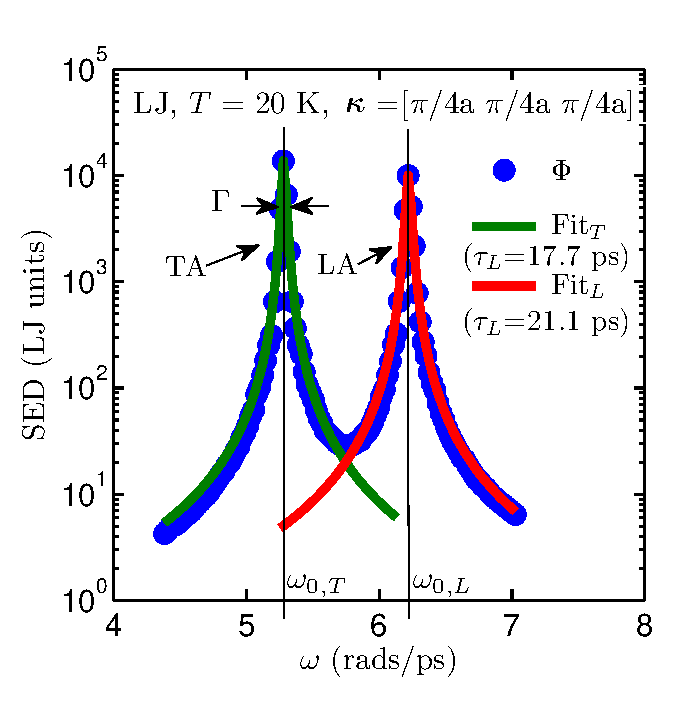
\includegraphics[angle=0,width=70.0mm]{LJ_FIT_PEAK.eps}
%\vspace*{-5mm}
%\end{center}
%\caption{\label{F:LJ_FIT_PEAK} The SED (using $\Phi$) for the first three polarizations at the wavevector $[\pi/4a,\pi/4a,\pi/4a]$ for LJ argon at a temperature of 20 K. There are two degenerate transverse acoustic polarizations and one longitudinal acoustic polarization (of higher frequency).\cite{dove1993} When fitting the SED, the different polarizations can be fit individually using single Lorentzian peaks or as a superposition of peaks. Here the two peaks are fit individually with $\Phi$ plotted as a superposition. The predicted lifetimes of these polarizations, which are inversely proportional to the peak widths $\Gamma$, are provided in the legend.}
%\end{figure}
%
%\vspace*{5mm}

\subsection{\label{Subsection_Comp_Details_3}Thermal Conductivity}

Once the frequencies and lifetimes of all phonon modes in the
Brillouin zone are obtained, the bulk thermal conductivity in direction
$\mathbf{n}$, $k_{\mathbf{n}}$, can be calculated from \cite{ziman2001}
\begin{equation}\label{E-size:k_bulk}\
\begin{split}
k_{\mathbf{n}}=&\sum_{\pmb{\kappa}} \sum_\nu c_{ph} \kv v^{2}_{g,\mathbf{n}} \kv \tau \kv.
\end{split}
\end{equation}
Here, $c_{ph}$ is the phonon volumetric specific heat and ${v}_{g,\mathbf{n}}$ is
the component of the group velocity vector in direction $\mathbf{n}$. Since the systems we consider are classical and obey Maxwell-Boltzmann statistics,\cite{mcquarrie2000} the
specific heat is $k_{B}/V$ per mode in the harmonic limit where $V$ is the system volume. This approximation is used here and has been shown to be suitable for LJ argon\cite{mcgaughey2004c} and SW silicon.\cite{goicochea2010} The group
velocity vector is the gradient of the dispersion curves (i.e., $\partial \omega / \partial \pmb{\kappa}$), which can be calculated from the frequencies and wavevectors using finite differences. In this work, the group velocities are calculated using finite difference and quasi-harmonic lattice dynamics because a very small finite difference can be used which reduces the error.\cite{mcgaughey2006b} To predict a bulk thermal conductivity, it is necessary to perform a finite simulation size scaling procedure as discussed in Appendix \ref{Appendix_C}.

\subsection{\label{Subsection_Comp_Details_3}Computational Cost}

The computational cost of evaluating Eq. \eqref{Lorentzian_SED} is less than that for Eq$.$ \eqref{E:ave_T_w1} by a factor of $3b$, where $b$ is the number of atoms in the unit cell.  For bulk crystals, the number of atoms in the unit cell is typically small ($b<10$).  In the CNT system, $b=32$ and evaluating $\Phi'$ is two orders of magnitude less expensive than evaluating $\Phi$.

To calculate the phonon lifetimes, the MD simulation time should be an order of magnitude longer than the longest phonon lifetime.\cite{thomasthesis}  If only the phonon frequencies are required, however, the location of the peaks in $\Phi$ and $\Phi'$ develop in a time on the order of the inverse of the phonon frequency, $1/\omega_0\kv$. For the systems studied here, this time to develop the peak locations can be two to five orders of magnitude less than the time needed to develop the lifetimes.

Fitting $\Phi'$ fitting becomes challenging at higher temperatures when the phonon linewidths broaden to become comparable to the spacing between mode frequencies. The cost of fitting $\Phi'$ can be reduced by fitting the peaks from all allowed wavevectors in the system simultaneously, but the error associated with this procedure is unknown.\cite{shiomi2011a} We find that a semi-automated procedure, whereby the fits are visualized, is necessary to ensure that all peaks are fit correctly.  While the computational cost of fitting $\Phi'$ is much smaller than the computational cost of calculating $\Phi'$, the semi-automated fitting procedure can be of similar time cost to the user. The cost of fitting $\Phi$ is much smaller because the different polarization peaks can be isolated and the fitting can be fully automated.

\section{\label{S:Section_Prop}Case Studies}

\subsection{\label{S:Subsection_prop_LJ}Lennard-Jones Argon}

We now use MD simulation to compare the SED calculated for LJ argon using $\Phi$ and $\Phi'$. The MD simulations are performed by LAMMPS.\cite{LAMMPS} We consider temperatures of 5, 20, and 40 K at zero-pressure with lattice constants of 5.278, 5.315 and 5.371 $\AA$. The normal mode method ($\Phi$) does lose accuracy
at higher temperatures because the quasi-harmonic phonon frequencies and
eigenvectors are used to perform the energy mapping
.\cite{turney2009a} A comparison between lattice dynamics (anharmonic lattice dynamics, $\Phi$) and MD (non-equilibrium direct-MD, equilibrium using Green-Kubo method) for LJ argon shows that lattice dynamics techniques start to diverge from the MD results for the thermal conductivity above half the melting temperature.\cite{turney2009a} In this paper, we limit the temperature to below half the melt temperature for all three systems studied. We are not testing lattice dynamics techniques but rather are comparing $\Phi$ and $\Phi'$.

The MD system consists of $N_1 \times N_2 \times N_3=512$ conventional cubic unit cells ($N_1=N_2=N_3=8$) for a total of 2048 atoms ($b=4$ atoms). Using a 4.285 fs time step, the system is equilibrated for $2^{20}$ time steps before collecting data every $2^5$ time steps for an additional $2^{20}$ time steps in the NVE ensemble.\cite{mcquarrie2000} The phonon frequencies, eigenvectors, and group velocities are generated under the quasi-harmonic lattice dynamics calculations using GULP.\cite{GULP} The sampling rate must be high enough to capture the highest phonon frequency in the system, which is determined {\em a priori} from quasi-harmonic lattice dynamics calculations. The sampling rate and total run time are chosen in powers of two as a convenience in performing fast Fourier transforms required to efficiently evaluate $\Phi$ and $\Phi'$. The same MD simulation data is used to calculate $\Phi$ and $\Phi'$.  Five simulations with different initial conditions are performed and the $\Phi$ and $\Phi'$ values are averaged before the peak fitting.

The SED ($\Phi$ and $\Phi'$) for the wavevector [$\pi/2a$,0,0] is presented in Fig$.$ \ref{F:PEAK_COMPARE} for all three temperatures. The edge of the Brioullin zone is at [$\pi/a$,0,0].  For $\Phi$, the spectral curve is plotted as a superposition over the twelve phonon polarizations. Degeneracy reduces the number of peaks to seven.  Overall, $\Phi'$ does not equal the total phonon spectral energy density $\Phi$, but the major features are similar. At all temperatures there are linewdith variations between the two spectral curves. We note that the linewidth (inverse lifetime) defined in Eq$.$ \eqref{E:ave_T_w1} is independent of the Lorentzian peak magnitude. The peak magnitudes become comparable for $\Phi$ and $\Phi'$ at high temperature.

The phonon frequencies and lifetimes extracted for all allowed wavectors in the first Brioullin zone using $\Phi$ and $\Phi'$ are compared on a mode-by-mode basis in Figs$.$ \ref{F:FREQ_LIFE_LJ}(a), \ref{F:FREQ_LIFE_LJ}(b), and \ref{F:FREQ_LIFE_LJ}(c). Here, $\omega$, $\omega^{'}$, $\tau$, and $\tau^{'}$  refer to the mode properties predicted using $\Phi$ and $\Phi'$. The phonon frequencies agree well at all three temperatures, with increasing scatter at high temperatures and high frequencies.  This scatter is due to the peak broadening seen in Fig$.$ \ref{F:PEAK_COMPARE}, which forces peaks close in frequency for $\Phi'$ to be fit as a single Lorentzian function and affects only high frequency peaks. For both $\Phi$ and $\Phi$, the predicted frequencies agree with those from quasi-harmonic lattice dynamics calculations to within less than five percent at $T=40$ K with better agreement at lower temperatures.  The agreement between $\Phi$ and $\Phi'$ in frequency is explained in Appendix \ref{Appendix_B}.

The lifetimes show large scatter between $\Phi$ and $\Phi'$ on a mode-by-mode basis, with increasing scatter at high temperature and no systematic difference. The scatter at high frequencies is due, in part, to the peak broadening seen in Fig$.$ \ref{F:PEAK_COMPARE}, which forces peaks close in frequency for $\Phi'$ to be fit as a single Lorentzian function with a single lifetime. The broadening does not affect fitting at low frequencies where the linewidths are much less than the peak spacings and the scatter comes solely from the disagreement between $\Phi$ and $\Phi'$.

The predicted phonon properties are then used to predict thermal conductivity using Eq$.$ \eqref{E-size:k_bulk}, presented in Table \ref{T:cond_table}. For LJ argon, a bulk thermal conductivity is predicted using a finite simulation size scaling procedure discussed in Appendix \ref{Appendix_C}. The bulk thermal conductivities predicted from $\Phi'$ are smaller and outside the uncertainty for those predicted from $\Phi$ for temperatures of $5$ and $20$ K. While the bulk thermal conductivities at a temperature of $40$ K agree within the uncertainty, the predicted mode-by-mode lifetimes show large scatter [Fig$.$ \ref{F:FREQ_LIFE_LJ}(c)] and the agreement should be regarded as coincidental. The uncertainties in the predicted thermal conductivities for $\Phi$ and $\Phi'$ come predominantly from the uncertainties in the finite size scaling procedure (Appendix \ref{Appendix_C}).

The disagreement between $\Phi$ and $\Phi'$ in thermal conductivity comes directly from the differences in the phonon lifetimes. All other properties (frequencies, group velocities, specific heats) are nearly or exactly the same for the two calculations. The bulk thermal conductivities predicted from $\Phi$ and $\Phi'$ are also compared to predictions from the Green-Kubo method. For $N_1=N_2=N_3=8$, the thermal conductivity predicted by the Green-Kubo method is converged with respect to the simulation size \cite{mcgaughey2004c}. The same MD data is used as the input for the Green-Kubo predictions. For all three temperatures, there is good agreement between $\Phi$ and Green-Kubo and the results for $\Phi$ and Green-Kubo are in good agreement with previous atomistic predictions\cite{turney2009a} using non-equilibrium direct-MD, anharmonic lattice dynamics, and $\Phi$.

%\begin{figure}
%\begin{center}
%\includegraphics[angle=0,width=80.0mm]{LJ_NMD_SED_PEAK_COMPARE.eps}
%\vspace*{-5mm}
%\end{center}
%\caption{\label{F:PEAK_COMPARE} The phonon spectral energy density ($\Phi$) is plotted as larger blue circles.  The proposed alternative expression for the phonon spectral energy density ($\Phi'$) is plotted as smaller green points. The wavevector is ($\pi/2a$,0,0) and the edge of the Brioullin zone is at ($\pi/a$,0,0).}
%\end{figure}
%
%\begin{figure}
%\begin{center}
%
%\subfigure{
%\includegraphics[angle=0,width=70.0mm]{LJ_NMD_SED_5K_2.eps}
%}
%\vspace*{-5mm}
%
%\subfigure{
%\includegraphics[angle=0,width=70.0mm]{LJ_NMD_SED_20K_2.eps}
%}
%\vspace*{-5mm}
%
%\subfigure{
%\includegraphics[angle=0,width=70.0mm]{LJ_NMD_SED_40K_2.eps}
%}
%\vspace*{-5mm}
%
%\end{center}
%\caption{\label{F:FREQ_LIFE_LJ} Comparison of the phonon frequencies and lifetimes predicted using $\Phi$ ($\omega,\tau$) and $\Phi'$ ($\omega^{'},\tau^{'}$) for LJ argon at temperatures of (a) 5 K, (b) 20 K, and (c) 40 K. The phonon frequencies agree well at all three temperatures, while the phonon lifetimes show large scatter.}
%\end{figure}
%
%\vspace*{20mm}

\subsection{\label{S:Subsection_prop_SW}Stillinger-Weber Silicon}

We next compare the phonon properties and thermal conductivity predicted from $\Phi$ and $\Phi'$ for SW silicon \cite{stillinger1985} at a temperature of $300$ K and zero pressure with a lattice constant of 5.430 $\AA$. The SW system is stiffer (larger phonon group velocities, frequencies, and lifetimes) than LJ argon and is an additional test to determine if there is a systematic error in the predictions from $\Phi'$. The MD simulations are performed by LAMMPS.\cite{LAMMPS} The MD system consists
of $N_1 \times N_2 \times N_3=216$ conventional unit cells ($N_1=N_2=N_3=6$) for a total of 1728 atoms ($b=8$ atoms).

Using a 0.5 fs timestep, the system is equilibrated for $2^{20}$ time steps before collecting data every $2^5$ time step for $2^{22}$ time steps in the NVE ensemble.\cite{mcquarrie2000} The phonon frequencies, eigenvectors, and group velocities are generated under the quasi-harmonic approximation using GULP.\cite{GULP} As for the LJ system, the sampling rate is determined by the highest phonon frequency in the system obtained {\em a priori} from quasi-harmonic lattice dynamics calculations. Five simulations with different initial conditions are performed and the $\Phi$ and $\Phi'$ values are averaged before the peak fitting.

The extracted phonon frequencies and lifetimes are plotted in Fig. \ref{F:FREQ_LIFE_Si}. As with the LJ system, the phonon frequencies are predicted accurately by $\Phi'$ but the lifetimes show large scatter on a mode-by-mode basis. For the system size studied, $\Phi'$ predicts a larger thermal conductivity than $\Phi$ outside the prediction uncertainties, in contrast to the LJ system (see Table \ref{T:cond_table}). The disagreement in thermal conductivity comes directly from the predicted phonon lifetimes. For SW silicon, a single system size is used since we are only interested in comparing the phonon properties predicted from $\Phi$ and $\Phi'$, and thus a bulk thermal conductivity is not predicted.

\subsection{\label{S:Subsection_prop_CNT}Carbon Nanotube}

Finally, we compare the phonon properties and thermal conductivies predicted by $\Phi$ and $\Phi'$ for an (8,8) CNT (diameter of 1.10-nm and a length of 12.3 nm) at a temperature of $300$ K and zero pressure.\cite{thomas2010c} The interactions in the CNT system are modeled using the reactive empirical
bond order (REBO) potential without the four-body interaction term.\cite{brenner2002} The MD simulations are performed by an in-house code.\cite{thomas2010c} The purpose of simulating this system is to check the results of Thomas $et al.$\cite{thomas2010c} and to compare the predictions of $\Phi'$ and $\Phi$. The MD system consists of $N_1 = N_2 = 1, N_3 = 50$ conventional unit cells ($b=32$ atoms) for a total of 1600 atoms.

Using a 1.0 fs timestep, the system is equilibrated for $2^{20}$ time steps before collecting data every $2^3$ time step for $2^{22}$ time steps in the NVE ensemble.\cite{mcquarrie2000} The phonon frequencies, eigenvectors, and group velocities are generated under the quasi-harmonic approximation using an in-house code.\cite{thomas2010c} As with the LJ and SW systems, the sampling rate is determined by the highest phonon frequency in the system obtained {\em a priori} from quasi-harmonic lattice dynamics calculations. Five simulations with different initial conditions are performed and the $\Phi$ and $\Phi'$ values are averaged before the peak fitting.

The phonon frequencies and lifetimes for the allowed wavevectors in the one dimensional Brioullin zone of the CNT are shown in Fig. \ref{F:FREQ_LIFE_CNT}. Like the LJ and SW silicon systems, the phonon frequencies can be predicted accurately by $\Phi'$, but the lifetimes show large scatter. The estimated thermal conductivity of the CNT predicted using $\Phi'$ is in good agreement with the results of Thomas $et al.$.\cite{thomas2010c} The thermal conductivity predicted by $\Phi'$ is less than that predicted by $\Phi$ but not outside the uncertainties.


%\begin{table}
%\caption{\label{T:cond_table}Thermal conductivity values in W/m-K predicted using $\Phi$, $\Phi'$, and the Green-Kubo methods.  The results for $\Phi$ and Green-Kubo are in good agreement with those of other atomistic simulation methods\cite{turney2009a} while $\Phi'$ differs and shows no systematic behavior.}
%\begin{ruledtabular}
%\begin{tabular}{llllll}
%     &                             &         &      &   \\
%$T$ (K)&Green-Kubo \ &$\Phi$ &$\Phi'$\\
%\hline
%LJ ($N_1=N_2=N_3=\infty$)\\
%5&8.0 $\pm$ 0.30 &7.9 $\pm$ 0.42 &5.8 $\pm$ 0.31 \\
%20&1.3 $\pm$ 0.15 &1.2 $\pm$ 0.07 &1.0 $\pm$ 0.10 \\
%40&0.45 $\pm$ 0.07 &0.47 $\pm$ 0.03 &0.49 $\pm$ 0.05 \\
%\hline
%SW ($N_1=N_2=N_3=6$) \\
%300& &530 $\pm$ 26 &651 $\pm$ 63 \\
%\hline
%CNT ($N_1=N_2=1, N_3=50$) \\
%300& &428 $\pm$ 21 &398 $\pm$ 40 \\
%\end{tabular}
%\end{ruledtabular}
%\end{table}


\section{\label{Section_Conclusions}Conclusions}

We derived the phonon spectral energy density, $\Phi$, and its relation to the phonon frequencies and lifetimes from the normal mode coordinates. We then presented an alternative formulation to the phonon spectral energy density, $\Phi'$, which does not require knowledge of the phonon eigenvectors.  Because $\Phi'$ does not contain the phonon eigenvectors, the alternative formulation does not represent the phonon spectral energy density but does contain information about the phonon frequencies as the temperature approaches $0$ K (see Appendix \ref{Appendix_B}).

We then calculated the phonon spectral energy density for LJ argon, SW silicon, and a CNT modeled with the REBO potential using $\Phi$ and $\Phi'$. The phonon frequencies and
lifetimes predicted from $\Phi$ and $\Phi'$ are shown in Figs$.$ \ref{F:FREQ_LIFE_LJ}, \ref{F:FREQ_LIFE_Si} and \ref{F:FREQ_LIFE_CNT}. The
frequencies are in excellent agreement between the two SED methods, while the lifetimes show large scatter.

The phonon SED $\Phi$ is well-defined theoretically,\cite{dove1993,wallace1972} while $\Phi'$ does not properly map the phonon energies since it is missing the phonon eigenvector. We deduce that this is the reason $\Phi'$ cannot accurately predict the phonon lifetimes. The three case studies in this work show that there is a systematic error in the lifetimes predicted from $\Phi'$. What is surprising is how close the predicted thermal conductivities can be using $\Phi$ and $\Phi'$.

Still, the most important properties predicted are the mody-by-mode phonon properties. Of particular importance are the lifetimes, which are the key input for Boltzmann transport equation-based models.\cite{mcgaughey2011a} Thus, we do not recommend $\Phi'$ for predicting phonon lifetimes or thermal conductivity.  Any agreement in thermal conductivity predictions from previous studies \cite{thomas2010c,dekoker2009,qiu2011} must be regarded as fortuitous. The phonon lifetime reductions in systems with additional scattering methods \cite{thomas2010c,shiomi2011a} can only be interpreted qualitatively. We recommend that $\Phi'$ be used for measuring phonon dispersion, as in the original formulation \cite{maruyama2003}, and the lifetime be interpreted correctly.

\begin{acknowledgments}
This work is supported by AFOSR award FA95501010098.
\end{acknowledgments}

\appendix
\section{\label{Appendix_A}Derivation of Phonon Spectral Energy Density}

We start from Eq$.$ \eqref{E:qdot_HLD}. In an anharmonic system, the phonon populations fluctuate about the
equilibrium distribution function.\cite{wallace1972} The phonon mode coordinate for the mode described by ($\nu,\pmb{\kappa}$) and its time
derivative can be written as\cite{dove1993}
\begin{equation}\label{A:E:q_A}
\begin{split}
q\kvt=&q_{SS}\kvt+q_{T}\kvt
\end{split}
\end{equation}
and
\begin{equation}\label{A:E:qdot_A}
\begin{split}
\dot{q}\kvt=& \dot{q}_{SS}\kvt+\dot{q}_{T}\kvt.
\end{split}
\end{equation}
The steady-state (SS) and transient (T) parts and their time derivatives are given by
\begin{equation}\label{A:E:q_A_SS}
\begin{split}
q_{SS}\kvt=& C_1\kv\exp[i\omega_0\kv t]
\\& +C_2\kv\exp[-i\omega_0\kv t],
\end{split}
\end{equation}
\begin{equation}\label{A:E:q_A_T}
\begin{split}
q_{T}\kvt=& \EXP{-\Gamma\kv |t|}\lbrace C_3\kv\EXP{i\omega_0\kv t}
\\ &-C_4\kv\EXP{-i\omega_0\kv t } \rbrace,
\end{split}
\end{equation}
\begin{equation}\label{A:E:qdot_A_SS}
\begin{split}
\dot{q}_{SS}\kvt=& i\omega_0\left\{C_1\kv\exp[i\omega_0\kv t]-C_2\kv\exp[-i\omega_0\kv t]\right\} ,
\end{split}
\end{equation}
and
\begin{equation}\label{E:qdot_A_T}
\begin{split}
\dot{q}_{T}\kvt=& \EXP{-\Gamma\kv |t|}\left\{C_3\kv\left[i\omega_0\kv-\Gamma\kv\right]\EXP{i\omega_0\kv t}\right. \\
& \left.-C_4\kv\left[i\omega_0\kv+\Gamma\kv\right]\EXP{-i\omega_0\kv t } \right\},
\end{split}
\end{equation}
where the $C$s are constants and $\omega_0\kv$ and $\Gamma\kv$ are the phonon
mode frequency and scattering rate (i$.$e$.$, linewidth).  The transient part
describes the creation of an excess in the population of a phonon mode for
$t<0$ and its decay back to equilibrium for $t>0$.

Phonon interactions arise due to anharmonicity, which causes fluctuations in the phonon populations. These population fluctuations are commonly modeled using the excitation and decay of
a single phonon mode (single mode relaxation time approximation).\cite{wallace1972,mcgaughey2004c}  In a real system, there will be multiple phonons in
each mode that simultaneously grow or decay with time.  Thus, dealing only
with $\dot{q}$, we let
\begin{equation}\label{A:E:qdot_A_kvbat}
\begin{split}
\dot{q}\kvt =& \sum_j i\EXP{-\Gamma\kv |t-t_j|}\times \\
& \lbrace A_j\kv\left[\omega_0\kv+i\Gamma\kv\right]\EXP{i\omega_0\kv (t-t_j)} \\
& -B_j\kv \left[\omega_0\kv-i\Gamma\kv\right]\EXP{-i\omega_0\kv (t-t_j) } \rbrace \\,
\end{split}
\end{equation}
where many phonons in each mode, indexed by $j$, are simultaneously being
created and destroyed.  The phonons grow for $t<t_j$ and decay for $t>t_j$
and $A_j$ and $B_j$ are constants.  We are  not concerned with the values of
$t_j$, $A_j$, and $B_j$, though they should satisfy the long-time average
$\langle\dot{q}_{SS}^*\kvt\dot{q}_{SS}\kvt\rangle=\langle\dot{q}^*\kvt\dot{q}\kvt\rangle$.

The expectation value of the kinetic energy of the normal coordinate is
\begin{equation}\label{A:E:ave_T_t}
\begin{split}
\langle T\kv \rangle=\frac{1}{2}\lim_{\tau_0\rightarrow\infty}\frac{1}{\tau_0}\int_{0}^{\tau_0}\dot{q}^*\kvt\dot{q}\kvt dt.
\end{split}
\end{equation}
This expression can be transformed from the time domain $t$ to the
frequency domain $\omega$ by Parseval's theorem,\cite{rudin1987}  allowing
Eq$.$ \eqref{A:E:ave_T_t} to be written as
\begin{equation}\label{A:E:ave_T_w1}
\begin{split}
T\kvw=\lim_{\tau_0\rightarrow\infty}\frac{1}{2\tau_0}\left|\frac{1}{\sqrt{2\pi}}\int_{0}^{\tau_0}\dot{q}\kvt\exp(-i\omega t)dt\right|^2.
\end{split}
\end{equation}
By substituting Eq$.$ \eqref{A:E:qdot_A_kvbat} into Eq$.$ \eqref{A:E:ave_T_w1} and performing the integration over time we find
\begin{equation}\label{A:E:ave_T_w_int}
\begin{split}
T\kvw = \frac{1}{16\pi\tau_0}\left|\sum_j\EXP{-i\omega t_j} \left\{A_j\kv\frac{\omega_0\kv+i\Gamma\kv}{\omega_0\kv-\omega+i\Gamma\kv}\right.\right.\\
\left.\left.+B_j\kv\frac{\omega_0\kv-i\Gamma\kv}{\omega_0\kv+\omega-i\Gamma\kv}\right\}\right|^2.
\end{split}
\end{equation}
We are primarily interested in values of $\omega$ where $\omega\approx\omega_0$ when $\Gamma<<\omega_0$ (this condition is met for the three systems studied here).  When $\omega\approx\omega_0$, the term involving $A_j$ becomes large and the term involving $B_j$ can be neglected (alternatively, we could ignore the term involving $A_j$ when $\omega\approx-\omega_0$).  Hence, we find
\begin{equation}\label{A:E:ave_T_w_approx}
\begin{split}
T\kvw=\frac{1}{16\pi\tau_0}\sum_j\sum_{j'}\cos\left[\omega (t_{j'}-t_j)\right]A_j\kv A_{j'}\kv\\
\times\frac{\omega_0^2\kv+\Gamma^2\kv}{\Gamma\kv}\frac{\Gamma\kv}{[\omega_0\kv-\omega]^2+\Gamma^2\kv}.
\end{split}
\end{equation}
We arrive at the expression for the phonon spectral energy density by summing Eq$.$ \eqref{A:E:ave_T_w_approx}
\begin{equation}\label{A:E:Lorentzian_NMD}
\begin{split}
\Phi(\omega,\pmb{\kappa}) = 2\sum_{\nu}^{3n} T\kvw=\sum_{\nu}^{3n}C_0\kv\frac{\Gamma\kv/\pi}{[\omega_0\kv-\omega]^2+\Gamma^2\kv},
\end{split}
\end{equation}
where the factor of two comes from equipartition of kinetic and potential energy (valid for a harmonic classical system, see Section \ref{Subsection_Comp_Details_3}), and
\begin{equation}\label{A:E:C_0}
\begin{split}
C_0\kv = \sum_j\sum_{j'}\cos\left[\omega (t_{j'}-t_j)\right]A_j\kv A_{j'}\kv\frac{\omega_0^2\kv+\Gamma^2\kv}{8\tau_0\Gamma\kv}.
\end{split}
\end{equation}
Thus, the phonon spectral energy density $\Phi(\omega,\pmb{\kappa})$ is a superposition of $3n$ Lorentzian
functions with centers at $\omega_0\kv$ (one for each polarization) with a half-width at half-maximum of
$\Gamma\kv$. $\Phi$ is a spectral energy density since its integral over all wavevectors and frequencies is the total crystal energy. The Hamiltonian can be written as
\begin{equation}\label{A:E:equipartition}
\begin{split}
H=\int\limits_{V_{BZ}} \int_{0}^{\infty}\Phi(\omega,\pmb{\kappa})d\omega d\pmb{\kappa},
\end{split}
\end{equation}
where $V_{BZ}$ is the volume of the Brioullin zone.  Like the broadening in frequency, there is also a broadening of the SED in wavevector.\cite{turneythesis} For a finite sampling of the Brioullin zone, the Hamiltonian can be written approximately as
\begin{equation}\label{A:E:equipartition}
\begin{split}
H \approx \sum_{\pmb{\kappa}}^N \int_{-\infty}^{\infty}\Phi(\omega,\pmb{\kappa})d\omega = 2\sum_{\pmb{\kappa},\nu}^{N,3n}\langle T\kvt\rangle.
\end{split}
\end{equation}

\section{\label{Appendix_B}Interpretation of $\Phi'$}

As demonstrated in Section \ref{S:Subsection_prop_LJ}, $\Phi'$ does not represent the phonon spectral energy density defined by Eq$.$ \eqref{E:ave_T_w1}. Our findings and those of others,\cite{maruyama2003,thomas2010c} however, suggest that $\Phi'$ does contain information about the phonon frequencies.  Under the harmonic approximation, the phonons are non-interacting and have no fluctuation in population (see Appendix \ref{Appendix}),
\begin{equation}\label{E:qdot_A_SS}
\begin{split}
\dot{q}\kvt =& \dot{q}_{SS}\kvt  \\
=& i\omega_0\kv\left\{C_1\kv\exp[i\omega_0\kv t]-C_2\kv\exp[-i\omega_0\kv t]\right\}.
 \end{split}
\end{equation}
Inserting Eq$.$ \eqref{E:qdot_A_SS} into the right hand side of Eq$.$ \eqref{SED} gives
\begin{equation}\label{Delta_SED}
\begin{split}
\sum_\alpha^3 \sum_b^n m_b \left| \sum_l^N  \int_{-\infty}^{\infty} \dot{u}_{\alpha}\lbt \EXP{i\pmb{\kappa}\cdot\mathbf{r}_0\ab{l}{0}-i\omega t} dt \right|^2 =& \\
\sum_\alpha^3 \sum_b^n\left| \frac{m_b^{3/2}}{\sqrt{N}} \sum_l^N \sum_{\nu}^{3n}  D\kvba \EXP{i\pmb{\kappa}\cdot\mathbf{r}_0\ab{l}{0}} \delta[ \omega_0\kv - \omega] \right|^2 ,
 \end{split}
\end{equation}
where $D\kvba = i\sqrt{2\pi} \omega_0\kv C_1\kv e^*\kvba$ and $\delta$ is the Dirac function. Thus, at zero temperature Eq$.$ \eqref{Lorentzian_SED} is a superposition of Dirac functions at the phonon frequencies $\omega_0\kv$.

\section{\label{Appendix_C}Finite Size Scaling}

The lifetimes are predicted in this work using $\Phi$ and $\Phi'$.  For the LJ argon system studied (Section \ref{S:Subsection_prop_LJ}), a finite simulation size scaling procedure\cite{turney2009a} is used to compare the predictions of $\Phi$ and $\Phi'$ to the Green-Kubo method.\cite{turney2009a} The scaling procedure is illustrated in Fig$.$ \ref{F:LJ_COND}.  The thermal conductivity is predicted from MD simulations with $N_0 = 4,6,8, and 10$. The bulk conductivity $k_{\infty}$, is then estimated by fitting the data to $1/k_{SED} = 1/k_{\infty} + A/N_0$, where $A$ is a constant.\cite{He2011} This procedure is necessary because the Brioullin zone is only sampled at a finite number of points. To predict a bulk value conductivity, it is important to properly sample points near the Brioullin zone center, where the modes have large lifetimes and group velocities and contribute significantly to thermal conductivty.\cite{turney2009a,sellan2010b} As with the predicted bulk thermal conductivities at temperatures of $5$ and $20$ K (Fig$.$ \ref{T:cond_table}, the predicted thermal conductivities at each system size ($N_0=4,6,8,10$) are systematically smaller for $\Phi'$.

%This method has been validated for non-equilibrium MD simulations \cite{sellan2010a}, but has not been validated for equilibrium MD.
\begin{figure}
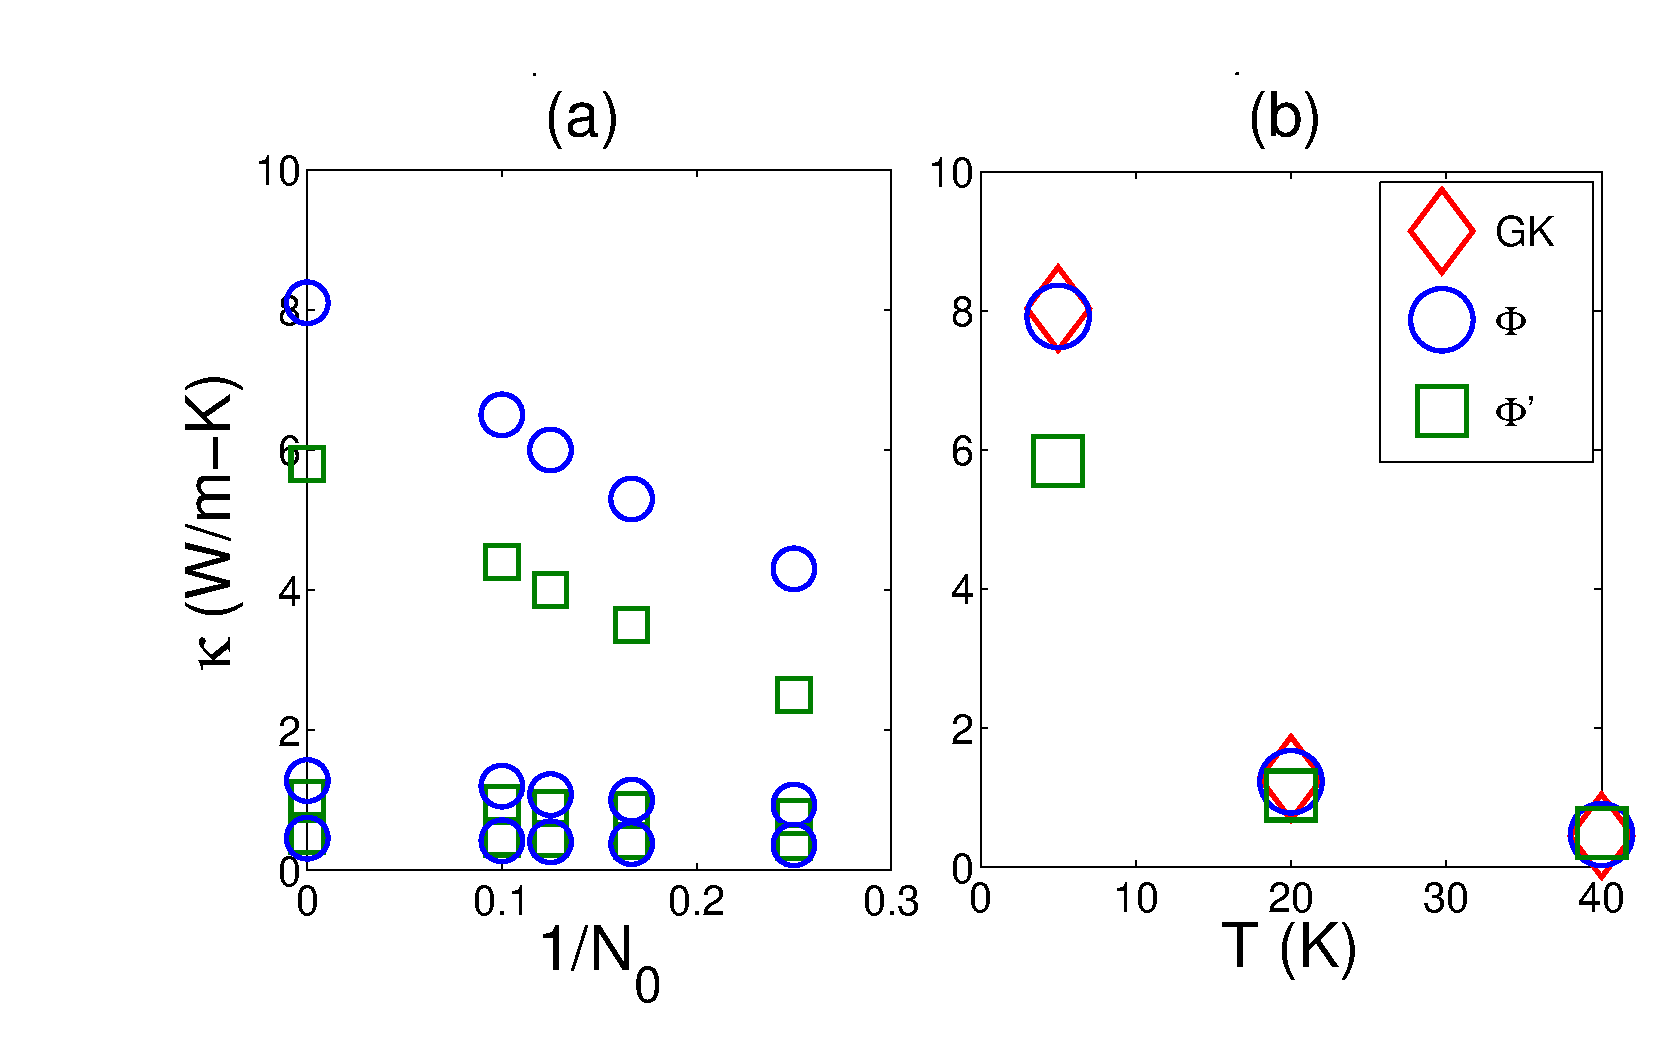
\includegraphics[angle=0,width=70.0mm]{LJ_NMD_SED_COND_2.eps}
\caption{\label{F:LJ_COND} Thermal conductivity predictions for LJ argon calculated using phonon lifetimes predicted by $\Phi$ and $\Phi'$. The finite size scaling extrapolation \cite{turney2009a,sellan2010a} is used to compare the results to bulk predictions made using the Green-Kubo method. The results for $\Phi$ and Green-Kubo are in good agreement with those of other atomistic simulation methods\cite{turney2009a}) while those from $\Phi'$ differ.}
\end{figure}

\vspace*{20mm}
\footnote[1]{When fitting the Lorentzian functions to $\Phi$ or $\Phi'$ the range of data must be selected. This range of data should be large enough for the Lorentzian functions to decrease significantly from their value at half-width at half-maximum (linewidth). The error in predicting the lifetime is obtained by varying this range of data used to fit the Lorentzian functions.}
% Create the reference section using BibTeX:
\bibliographystyle{apsrev}
\bibliography{references_thesis_proposal}

\end{document}
%
% ****** End of file ******
